\documentclass[aspectratio=169]{beamer}

\setbeamersize{text margin left=5mm, text margin right=5mm}

\defbeamertemplate{headline}{my header}{%
\vskip1pt%
\makebox[0pt][l]{\,\insertshortauthor}%
\hspace*{\fill}\insertshorttitle/\insertshortsubtitle\hspace*{\fill}%
\llap{\insertpagenumber/\insertpresentationendpage\,}
}
\setbeamertemplate{headline}[my header]

\let\olditem\item
\renewcommand{\item}{\setlength{\itemsep}{\fill}\olditem}

\usepackage{caption}
\usepackage{soul}
\usepackage{tkz-euclide}
\usetikzlibrary{calc}
\usepackage[]{algorithm2e}
\usepackage{changepage}
\usepackage{amssymb}
\usepackage{xcolor}
\usepackage{mathtools}
\usepackage{tcolorbox}
\usepackage{tikz}
\usepackage{tikz-3dplot}
\usepackage{tkz-euclide}
\usepackage{circuitikz}
\usepackage{mleftright}
\usetikzlibrary{arrows.meta, decorations.pathreplacing, positioning, shapes.geometric}

%% Fonts
\usefonttheme{professionalfonts}
\usefonttheme{serif}

\DeclareCaptionLabelFormat{blank}{}
\captionsetup[figure]{labelformat=blank}

%% Math definitions
\def\mf{\ensuremath\mathbf}
\def\mb{\ensuremath\mathbb}
\def\mc{\ensuremath\mathcal}
\def\lp{\ensuremath\left(}
\def\rp{\ensuremath\right)}
\def\lv{\ensuremath\left\lvert}
\def\rv{\ensuremath\right\rvert}
\def\lV{\ensuremath\left\lVert}
\def\rV{\ensuremath\right\rVert}
\def\lc{\ensuremath\left\{}
\def\rc{\ensuremath\right\}}
\def\ls{\ensuremath\left[}
\def\rs{\ensuremath\right]}
\def\bmx{\ensuremath\begin{bmatrix*}[r]}
\def\emx{\ensuremath\end{bmatrix*}}
\def\bmxc{\ensuremath\begin{bmatrix*}[c]}
\def\t{\lp t\rp}
\def\k{\ls k\rs}

\newcommand{\demoex}[2]{\onslide<#1->\begin{color}{black!60} #2 \end{color}}
\newcommand{\demoexc}[3]{\onslide<#1->\begin{color}{#2} #3 \end{color}}
\newcommand{\anim}[3]{\onslide<#1->{\begin{color}{#2!60} #3 \end{color}}}
\newcommand{\ct}[1]{\lp #1\rp}
\newcommand{\dt}[1]{\ls #1\rs}
\newcommand{\cols}[2]{\begin{columns}[#1] #2 \end{columns}}
\newcommand{\col}[2]{\begin{column}{#1} #2 \end{column}}

%% Mycolors
\definecolor{myred}{RGB}{192,0,0}
\definecolor{mygray}{RGB}{100,100,100}

%% Custom beamer color
\setbeamercolor{title}{fg=myred}
\setbeamercolor{subtitle}{fg=myred}
\setbeamerfont{title}{series=\bfseries}
% \setbeamercolor{frametitle}{bg=myred, fg=white}
\setbeamercolor{frametitle}{bg=mygray!10!, fg=myred}
\setbeamerfont{frametitle}{series=\bfseries}
\setbeamercolor{item}{fg=mygray}
\setbeamercolor{title in head/foot}{fg=myred}

% Move header to footer
\setbeamertemplate{headline}{}
\setbeamertemplate{footline}{
  \begin{beamercolorbox}[wd=\paperwidth,ht=2.25ex,dp=1ex,center]{footline}
    \inserttitle\hfill\insertauthor\hfill\insertdate\hfill\insertframenumber{}
  \end{beamercolorbox}
}


\title{Applied Linear Algebra for Data Analysis}

% A subtitle is optional and this may be deleted
\subtitle{Eigenvalues and Eigenvectors}

\author{Sivakumar Balasubramanian}
% - Give the names in the same order as the appear in the paper.
% - Use the \inst{?} command only if the authors have different
%   affiliation.

\institute[Christian Medical College] % (optional, but mostly needed)
{
  \inst{}%
  Department of Bioengineering\\
  Christian Medical College, Bagayam\\
  Vellore 632002
}
% - Use the \inst command only if there are several affiliations.
% - Keep it simple, no one is interested in your street address.

\date{}
% - Either use conference name or its abbreviation.
% - Not really informative to the audience, more for people (including
%   yourself) who are reading the slides online

\subject{Lecture notes on linear systems}
% This is only inserted into the PDF information catalog. Can be left
% out. 

% If you have a file called "university-logo-filename.xxx", where xxx
% is a graphic format that can be processed by latex or pdflatex,
% resp., then you can add a logo as follows:

% \pgfdeclareimage[height=0.5cm]{university-logo}{university-logo-filename}
% \logo{\pgfuseimage{university-logo}}

% Delete this, if you do not want the table of contents to pop up at
% the beginning of each subsection:
\AtBeginSubsection[]
{
  \begin{frame}<beamer>{Outline}
    \tableofcontents[currentsection,currentsubsection]
  \end{frame}
}

% Let's get started
\begin{document}

% \pgfplotsset{
%   compat=1.8,
%   colormap={whitered}{color(0cm)=(white); color(1cm)=(orange!75!red)}
% }


\begin{frame}
  \titlepage
\end{frame}


\begin{frame}[t]{Linear transformation}
\begin{itemize}
    \item Matrices represent linear transformations, $\mf{A} \in \mb{R}^{m \times n}$ represents a transformation $T: \mb{R}^n \to \mb{R}^m$. 
    \[ \mf{y} = T\left(\mf{x}\right) = \mf{A}\mf{x}, \,\,\,\, \mf{x} \in \mb{R}^n \text{ and } \, \mf{y} \in \mb{R}^m \]

    \item Consider a linear transformation $T: \mb{R}^n \to \mb{R}^n$.

    In general, $T$ scales, and rotates/reflects the vector $\mf{x}$ to produce $\mf{y}$.

    \begin{center}
    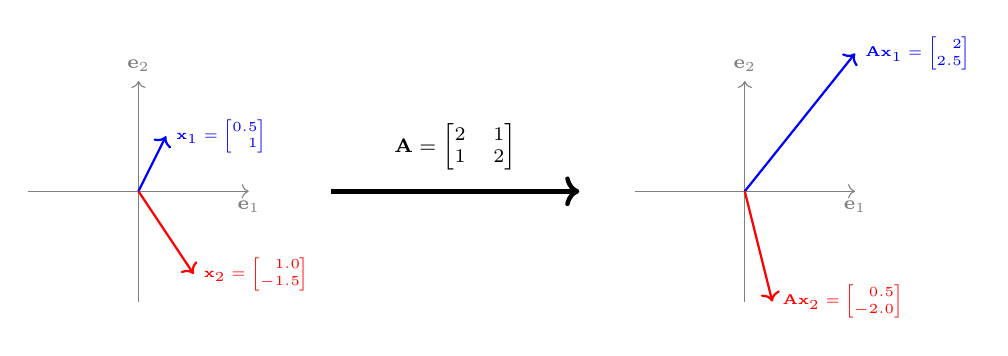
\begin{tikzpicture}[scale=0.7]
    \draw[thin, gray, ->] (-2,0) -- (2, 0) node[below] {\scriptsize{$\mf{e}_1$}};
    \draw[thin, gray, ->] (0, -2) -- (0, 2) node[above] {\scriptsize{$\mf{e}_2$}};
    \draw[thick, blue, ->] (0, 0) -- (0.5, 1) node[right] {\tiny{$\mf{x}_1 = \begin{bmatrix*}[r]0.5\\1\end{bmatrix*}$}};
    \draw[thick, red, ->] (0, 0) -- (1, -1.5) node[right] {\tiny{$\mf{x}_2 = \begin{bmatrix*}[r]1.0\\-1.5\end{bmatrix*}$}};

    \draw[ultra thick, black, ->] (3.5, 0) -- (8.0, 0);

    \node[black, above] at (5.75, 0.2) {\scriptsize{$\mf{A} = \begin{bmatrix*}2 & 1\\1 & 2\end{bmatrix*}$}};

    \draw[thin, gray, ->] (9,0) -- (13, 0) node[below] {\scriptsize{$\mf{e}_1$}};
    \draw[thin, gray, ->] (11, -2) -- (11, 2) node[above] {\scriptsize{$\mf{e}_2$}};
    \draw[thick, blue, ->] (11, 0) -- (13, 2.5) node[right] {\tiny{$\mf{A}\mf{x}_1 = \begin{bmatrix*}[r]2\\2.5\end{bmatrix*}$}};
    \draw[thick, red, ->] (11, 0) -- (11.5, -2.0) node[right] {\tiny{$\mf{A}\mf{x}_2 = \begin{bmatrix*}[r]0.5\\-2.0\end{bmatrix*}$}};
    \end{tikzpicture}
    \end{center}

\end{itemize}
\end{frame}


\begin{frame}[t]{Linear transformation}

{\small{An easier way is to look at what happens to the standard basis $\left\{\mf{e}_i\right\}_{i=1}^{n}$.}}

\begin{center}
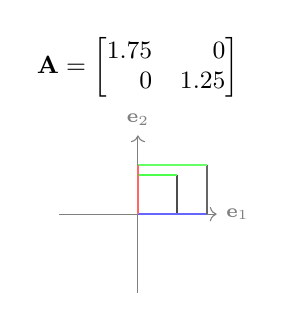
\begin{tikzpicture}[scale=0.5]
\draw[thin, gray, ->] (-2,0) -- (2, 0) node[right] {\scriptsize{$\mf{e}_1$}};
\draw[thin, gray, ->] (0, -2) -- (0, 2) node[above] {\scriptsize{$\mf{e}_2$}};

\draw[thick, blue!70!, -] (0, 0) -- (1, 0);
\draw[thick, black!70!, -] (1, 0) -- (1, 1);
\draw[thick, green!70!, -] (1, 1) -- (0, 1);
\draw[thick, red!70!, -] (0, 1) -- (0,0);
\draw[thick, blue!60!, -] (0, 0) -- (1.75, 0);
\draw[thick, black!60!, -] (1.75, 0) -- (1.75, 1.25);
\draw[thick, green!60!, -] (1.75, 1.25) -- (0, 1.25);
\draw[thick, red!60!, -] (0, 1.25) -- (0, 0);

\node[below, black] at (0.0, 4.75) {\small{$\mf{A} = \begin{bmatrix*}[r]1.75 & 0\\0 & 1.25\end{bmatrix*}$}};
\end{tikzpicture} \hspace{0.1cm}
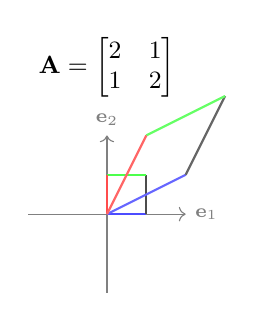
\begin{tikzpicture}[scale=0.5]
\draw[thin, gray, ->] (-2,0) -- (2, 0) node[right] {\scriptsize{$\mf{e}_1$}};
\draw[thin, gray, ->] (0, -2) -- (0, 2) node[above] {\scriptsize{$\mf{e}_2$}};

\draw[thick, blue!70!, -] (0, 0) -- (1, 0);
\draw[thick, black!70!, -] (1, 0) -- (1, 1);
\draw[thick, green!70!, -] (1, 1) -- (0, 1);
\draw[thick, red!70!, -] (0, 1) -- (0,0);
\draw[thick, blue!60!, -] (0, 0) -- (2, 1);
\draw[thick, black!60!, -] (2, 1) -- (3, 3);
\draw[thick, green!60!, -] (3, 3) -- (1, 2);
\draw[thick, red!60!, -] (1, 2) -- (0, 0);

\node[below, black] at (0.0, 4.75) {\small{$\mf{A} = \begin{bmatrix*}2 & 1\\1 & 2\end{bmatrix*}$}};
\end{tikzpicture} \hspace{0.1cm}
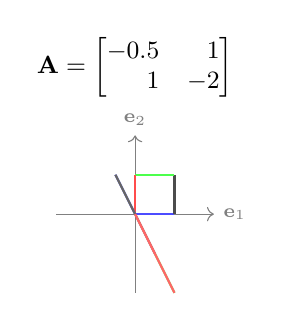
\begin{tikzpicture}[scale=0.5]
\draw[thin, gray, ->] (-2,0) -- (2, 0) node[right] {\scriptsize{$\mf{e}_1$}};
\draw[thin, gray, ->] (0, -2) -- (0, 2) node[above] {\scriptsize{$\mf{e}_2$}};

\draw[thick, blue!70!, -] (0, 0) -- (1, 0);
\draw[thick, black!70!, -] (1, 0) -- (1, 1);
\draw[thick, green!70!, -] (1, 1) -- (0, 1);
\draw[thick, red!70!, -] (0, 1) -- (0,0);
\draw[thick, blue!60!, -] (0, 0) -- (-0.5, 1);
\draw[thick, black!60!, -] (-0.5, 1) -- (0.5, -1);
\draw[thick, green!60!, -] (0.5, -1) -- (1, -2);
\draw[thick, red!60!, -] (1, -2) -- (0, 0);

\node[below, black] at (0.0, 4.75) {\small{$\mf{A} = \begin{bmatrix*}[r]-0.5 & 1\\1 & -2\end{bmatrix*}$}};
\end{tikzpicture} \hspace{0.1cm}
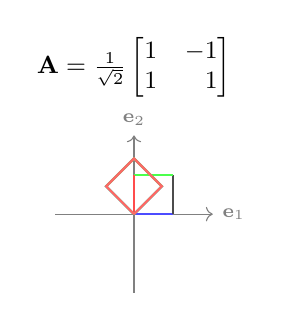
\begin{tikzpicture}[scale=0.5]
\draw[thin, gray, ->] (-2,0) -- (2, 0) node[right] {\scriptsize{$\mf{e}_1$}};
\draw[thin, gray, ->] (0, -2) -- (0, 2) node[above] {\scriptsize{$\mf{e}_2$}};

\draw[thick, blue!70!, -] (0, 0) -- (1, 0);
\draw[thick, black!70!, -] (1, 0) -- (1, 1);
\draw[thick, green!70!, -] (1, 1) -- (0, 1);
\draw[thick, red!70!, -] (0, 1) -- (0,0);
\draw[thick, blue!60!, -] (0, 0) -- (0.707, 0.707) -- (0, 1.414) -- (-0.707, 0.707) -- (0, 0);
\draw[thick, black!60!, -] (0, 0) -- (0.707, 0.707) -- (0, 1.414) -- (-0.707, 0.707) -- (0, 0);
\draw[thick, green!60!, -] (0, 0) -- (0.707, 0.707) -- (0, 1.414) -- (-0.707, 0.707) -- (0, 0);
\draw[thick, red!60!, -] (0, 0) -- (0.707, 0.707) -- (0, 1.414) -- (-0.707, 0.707) -- (0, 0);


\node[below, black] at (0.0, 4.75) {\small{$\mf{A} = \frac{1}{\sqrt{2}}\begin{bmatrix*}[r]1 & -1\\1 & 1\end{bmatrix*}$}};
\end{tikzpicture} \hspace{0.1cm}
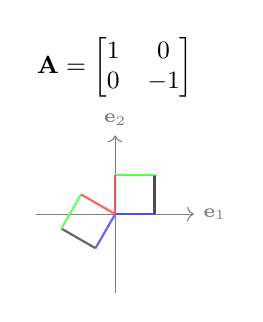
\begin{tikzpicture}[scale=0.5]
\draw[thin, gray, ->] (-2,0) -- (2, 0) node[right] {\scriptsize{$\mf{e}_1$}};
\draw[thin, gray, ->] (0, -2) -- (0, 2) node[above] {\scriptsize{$\mf{e}_2$}};

\draw[thick, blue!70!, -] (0, 0) -- (1, 0);
\draw[thick, black!70!, -] (1, 0) -- (1, 1);
\draw[thick, green!70!, -] (1, 1) -- (0, 1);
\draw[thick, red!70!, -] (0, 1) -- (0,0);
\draw[thick, blue!60!, -] (0, 0) -- (-0.5, -0.866);
\draw[thick, black!60!, -] (-0.5, -0.866) -- (-1.366, -0.366);
\draw[thick, green!60!, -] (-1.366, -0.366) -- (-0.866, 0.5);
\draw[thick, red!60!, -] (-0.866, 0.5) -- (0, 0);

\node[below, black] at (0.0, 4.75) {\small{$\mf{A} = \begin{bmatrix*}1 & 0\\0 & -1\end{bmatrix*}$}};
\end{tikzpicture}
\end{center}

\end{frame}


\begin{frame}[t]{Linear transformation in different basis}
\begin{itemize}
    \item Consider a basis $V=\left\{\mf{v}_i\right\}_{i=1}^{n}$ for $\mb{R}^n$. Let $\mf{x} = \begin{bmatrix*}x_1 & x_2 & \ldots & x_n\end{bmatrix*}^\top \in \mb{R}^n$ be the representation of $\mf{x}$ in 
    the standard basis.
    
    Representation of $\mf{x}$ in $V$ is,
    \[ \mf{x} = \sum_{i=1}^n x_{vi}\mf{v}_i, \,\,\, \mf{x}_V = \begin{bmatrix*}x_{v1} & x_{v2} & \ldots & x_{vn}\end{bmatrix*}^\top \]

    \item We can go back and forth between these two representations in the following way,
    \[ \mf{x} = \mf{V}\mf{x}_V \,\,\, \text{ and } \,\,\, \mf{x}_V = \mf{V}^{-1}\mf{x}; \,\,\, \text{where, } \mf{V} = \begin{bmatrix*}\mf{v}_1 & \mf{v}_2 & \ldots & \mf{v}_n\end{bmatrix*} \]

    \item When $V$ is an orthonormal basis, then the algebra gets simpler,
    \[ \mf{x} = \mf{V}\mf{x}_V \,\,\, \text{ and } \,\,\, \mf{x}_V = \mf{V}^\top\mf{x} \]

\end{itemize}
\end{frame}


\begin{frame}[t]{Linear transformation in different basis}
\begin{small}
Consider a linear transformation $T: \mb{R}^2 \to \mb{R}^2$ represented by the matrix $\mf{A} = \begin{bmatrix*}[r]1 & 0\\-1 & 1\end{bmatrix*}$. Consider a vector $\mf{x} = \begin{bmatrix*}[r]2\\-1\end{bmatrix*}$. What is $\mf{y} = \mf{Ax}$?

\[ \mf{y} = \mf{Ax} = \begin{bmatrix*}[r]1 & 0\\-1 & 1\end{bmatrix*}\begin{bmatrix*}[r]2\\-1\end{bmatrix*} = \begin{bmatrix*}[r]2\\-3\end{bmatrix*} \]

Now, consider a basis $V = \left\{\begin{bmatrix*}[r]1\\-1\end{bmatrix*}, \begin{bmatrix*}[r]2\\1\end{bmatrix*}\right\}$ for $\mb{R}^2$. The representation of $\mf{x}, \mf{y}$ in $V$ is, 

\[ \mf{x}_V = \mf{V}^{-1}\mf{x} = \frac{1}{3}\begin{bmatrix*}[r]1 & -2\\1 & 1\end{bmatrix*}\begin{bmatrix*}[r]2\\-1\end{bmatrix*} = \frac{1}{3}\begin{bmatrix*}[r]4\\1\end{bmatrix*}, \,\,\, \mf{y}_V = \mf{V}^{-1}\mf{y} = \frac{1}{3}\begin{bmatrix*}[r]8\\-1\end{bmatrix*}\]

Now, if we apply the linear transformation $T$ on $\mf{x}_V$ will we get $\mf{y}_V$?

\[ \mf{A}\mf{x}_V = \begin{bmatrix*}[r]1 & 0\\-1 & 1\end{bmatrix*}\frac{1}{3}\begin{bmatrix*}[r]-4\\1\end{bmatrix*} = \frac{1}{3}\begin{bmatrix*}[r]-4\\5\end{bmatrix*} \neq \mf{y}_V \]

\textbf{Representation of a linear transformation $T$ is basis dependent! }
\end{small}

\end{frame}


\begin{frame}[t]{Similarity transformation}
\begin{itemize}
    \item Linear transformations represented in one basis represent a different transformation in another basis. This issue can be addressed by keeping track of the basis one is working in.

    \item Let $\mf{x}, \mf{y}$ be representations in the standard basis. Changing basis to $V$, gives us $\mf{x}_V, \mf{y}_V$.
    \[ \mf{y}_V = \mf{V}^{-1}\mf{y} = \mf{V}^{-1}\mf{Ax} = \mf{V}^{-1}\mf{A}\mf{V}\mf{x}_V = \mf{A}_V\mf{x}_V \]
\end{itemize}
\end{frame}


% \begin{frame}[t]{Similarity transformation}
% \begin{itemize}
%     \item Check if this works with the example in the previous slide. $\mf{A} = \begin{bmatrix*}[r]1 & 0\\-1 & 1\end{bmatrix*}$; $\mf{V} = \begin{bmatrix*}[r]1 & 2\\-1 & 1\end{bmatrix*}$. Determine $\mf{A}_V$ and check that $\mf{y}_V = \mf{A}_V\mf{x}_V$.

% \end{itemize}
% \end{frame}


% \begin{frame}[t]{Similarity transformation}
% \begin{itemize}
%     \item A linear transformation $\hat{T}$ is represented as $\mf{A}_V$ in $V$. What is its representation in the standard basis? E.g.: $\mf{A}_V = \begin{bmatrix*}[r]-4 & 1\\1 & 2\end{bmatrix*}$; $\mf{V} = \frac{1}{\sqrt{2}}\begin{bmatrix*}[r]1 & 1\\-1 & 1\end{bmatrix*}$. Determine $\mf{A}$. If $\mf{x}_V = \bmx \frac{1}{2} & 2\emx^\top$. What is $\mf{y}_V$ and $\mf{y}$?
% \end{itemize}
% \end{frame}


\begin{frame}[t]{Similarity transformation}
\begin{itemize}
    \item Two matrices $\mf{A}, \mf{B} \in \mb{R}^{n \times n}$ are called \textit{similar} matrices, if there exists a non-singular matrix $\mf{Q}$, such that,
    \[ \mf{B} = \mf{Q}^{-1}\mf{A}\mf{Q} \]

    \item The transformation represented by $\mf{Q}^{-1}\mf{A}\mf{Q}$ is called the \textit{similarity transformation}.

    \item \textit{Similar} matrices represent the same linear transformation in different basis.

    \item When $\mf{Q}$ is an orthogonal matrix, we have $\mf{B} = \mf{Q}^\top\mf{A}\mf{Q}$. 
\end{itemize}
\end{frame}


\begin{frame}[t]{Eigenvectors and Eigenvalues}
\begin{itemize}
    \item Any linear transformation represented by $\mf{A} \in \mb{C}^{n \times n}$ has vectors that satisfy the following property,
    \[ \mf{Ax} = \lambda \mf{x}, \,\,\,\,\, \mf{x} \in \mb{C}^n, \, \lambda \in \mb{C}, \,\,\, \mf{x} \neq \mf{0} \]
    where, $\lambda$ and $\mf{x}$ are called the eigenvalue and the associated eigenvector of $\mf{A}$.
    
    \item Any such pair $\left(\lambda, \mf{x}\right)$ is called the eigenpair of $\mf{A}$.
    
    \item These are important for understanding and solving linear differential and difference equations:
    \[ \frac{d\mf{x}\left(t\right)}{dt} = \mf{A}\mf{x}\left(t\right) \,\,\, \text{ and } \,\,\, \mf{x}\left[n+1\right] = \mf{A}\mf{x}\left[n\right] \]
\end{itemize}
\end{frame}


\begin{frame}[t]{Eigenvectors and Eigenvalues}
Consider the differential equation, $\frac{d\mf{x}\left(t\right)}{dt} = \mf{A}\mf{x}\left(t\right) = \begin{bmatrix*}-5 & 11\\0 & -6\end{bmatrix*}\mf{x}\left(t\right)$. Let us assume that the solution is of the form, $\mf{x} = e^{\lambda t}\hat{\mf{x}}$. Then we have,
\[ \frac{d\mf{x}\left(t\right)}{dt} = e^{\lambda t}\mf{A}\hat{\mf{x}} = e^{\lambda t} \lambda \hat{\mf{x}} \implies \mf{A}\hat{\mf{x}} = \lambda \hat{\mf{x}} \]
\[ \begin{bmatrix*}-5 & 11\\0 & -6\end{bmatrix*}\begin{bmatrix*}\hat{x}_1\\\hat{x}_2\end{bmatrix*} = \begin{bmatrix*}\lambda \hat{x}_1\\\lambda \hat{x}_2\end{bmatrix*} \implies \begin{bmatrix*}-5 - \lambda & 11\\0 & -6 - \lambda\end{bmatrix*}\begin{bmatrix*}\hat{x}_1\\\hat{x}_2\end{bmatrix*} = \begin{bmatrix*}0\\0\end{bmatrix*} \]
where, $\hat{\mf{x}} \in N\left(\mf{A} - \lambda\mf{I}\right)$.
\end{frame}


\begin{frame}{Eigenvalues and Eigenvectors}
\begin{itemize}
    \item We can find the eigenpairs using the same approach for $\mf{A} \in \mb{C}^{n \times n}$, $\det \left(\mf{A} - \lambda\mf{I}\right) = 0 = p\left(\lambda\right)$.

    \item $p\left(\lambda\right)$ is the characteristic polynomial of $\mf{A}$, and $p\left(\lambda\right) = 0$ is the characteristic equation.

    \item The eigenvalues are the roots of the polynomial $p\left(\lambda \right)$, and the $\mf{x}$ in $\left(\mf{A} - \lambda\mf{I}\right)\mf{x} = 0$ for the different $\lambda$s are the corresponding eigenvectors. 
\end{itemize}
\end{frame}


\begin{frame}[t]{Eigenvalues and Eigenvectors}
Compute the eigenpairs for the following matrices: $\bmx2 & 1\\-1 & 3\emx$, $\bmx1 & 0\\0 & 1\emx$, $\bmx2 & 1\\ 1 & 2\emx$.
\end{frame}


\begin{frame}[t]{Eigenvalues and Eigenvectors}
Compute the eigenpairs for the following matrices: $\bmx\frac{\sqrt{3}}{2} & \frac{1}{2}\\-\frac{1}{2} & \frac{\sqrt{3}}{2}\emx$, $\bmx 0 & -2\\2 & 0\emx$.
\end{frame}


\begin{frame}[t]{Diagonalization of a matrix}

Often the right choice of basis can simplify an equation or the analysis of a problem. For example,
\begin{columns}
\begin{column}{0.5\textwidth}
    \begin{center}
        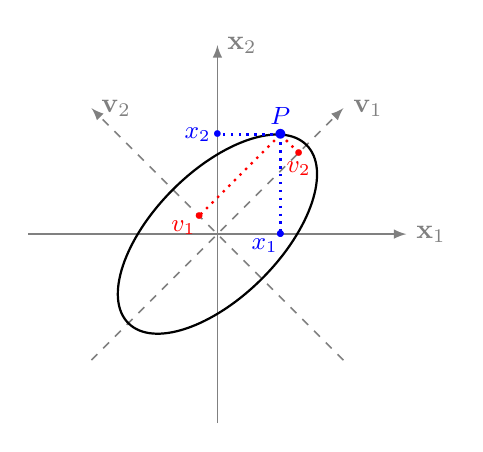
\begin{tikzpicture}[scale=0.8]
        \draw[gray, -latex, line width=0.2mm] (-3, 0) -- (3, 0) node[right] {$\mf{x}_1$};
        \draw[gray, -latex, line width=0.2mm] (0, -3) -- (0, 3) node[right] {$\mf{x}_2$};
        \draw[gray, dashed, -latex, line width=0.2mm] (-2, -2) -- (2, 2) node[right] {$\mf{v}_1$};
        \draw[gray, dashed, -latex, line width=0.2mm] (2, -2) -- (-2, 2) node[right] {$\mf{v}_2$};
        \draw[thick, rotate=45] (0,0) ellipse (2 and 1);
        \node[blue, above] at (1, 1.579795) {\small{${P}$}};
        \draw[blue, dotted, line width=0.3mm] (1, 1.579795) -- (1, 0) node[blue, yshift=-0.15cm, xshift=-0.2cm] {\small{$x_1$}};
        \node[blue] at (1, 0) {\tiny{$\bullet$}};
        \draw[blue, dotted, line width=0.3mm] (1, 1.579795) -- (0, 1.579795) node[blue, xshift=-0.25cm, yshift=0.cm] {\small{$x_2$}}; 
        \node[blue] at (0, 1.579795) {\tiny{$\bullet$}};
        \draw[red, dotted, line width=0.3mm] (1, 1.579795) -- (-0.289892, 0.289892) node[red, yshift=-0.15cm, xshift=-0.2cm] {\small{$v_1$}};
        \node[red] at (-0.289892, 0.289892) {\tiny{$\bullet$}};
        \draw[red, dotted, line width=0.3mm] (1, 1.579795) -- (1.289897, 1.289897) node[red, yshift=-0.2cm, xshift=0.0cm] {\small{$v_2$}};
        \node[blue] at (1, 0) {\tiny{$\bullet$}};
        \node[red] at (1.289897, 1.289897) {\tiny{$\bullet$}};
        \node[blue] at (1, 1.579795) {\small{$\bullet$}};
        % \draw[blue, dotted, line width=0.5mm] (1, 1.579795) -- (0, 1.579795); 
        \end{tikzpicture}
    \end{center}
\end{column}
\begin{column}{0.5\textwidth}
The equation of the ellipse in standard basis is: 
\[ 3x_1^2 + 3x_2^2 - 2x_1x_2 = 1 \]

This has a much simpled representation in the dashed coordinate frame. 
\[ 4v_1^2 + 2v_2^2 = 1 \]

The use of similarity transformation to simplify a matrix is at the heart of diagonalization.
\end{column}
\end{columns}
\end{frame}


\begin{frame}[t]{Diagonalization of a matrix}
\begin{itemize}
    \item Consider a matrix $\mf{A}$ with $n$ eigenpairs $\left\{\left(\lambda_i, \mf{x}_i\right)\right\}_{i=1}^n$.
    \[ \mf{A}\begin{bmatrix*}\mf{x}_1 & \mf{x}_2 & \ldots & \mf{x}_n\end{bmatrix*} = \begin{bmatrix*}\lambda_1\mf{x}_1 & \lambda_2\mf{x}_2 & \ldots & \lambda_n\mf{x}_n\end{bmatrix*} \]
    \[ \mf{AX} = \mf{X}\begin{bmatrix*}\lambda_1 & 0 & \ldots & 0\\0 & \lambda_2 & \ldots & 0\\\vdots & \vdots & \ddots & \vdots\\0 & 0 & \ldots & \lambda_n\end{bmatrix*} = \mf{X}\mf{\Lambda} \]

    \item If the eignevectors are linearly independent, then we have $\mf{X}^{-1}\mf{A}\mf{X} = \mf{\Lambda}$
\end{itemize}
\end{frame}


\begin{frame}[t]{Diagonalization of a matrix}
Let $T: \mb{R}^2 \to \mb{R}^2$ represented by $\mf{A} = \bmx 8 & 1\\2 & 7\emx$. Diagonalize this matrix. What does $\mf{A}$ do to $\mf{x} = \bmx 3 & 4\emx^\top$?
\end{frame}


\begin{frame}[t]{Diagonalization of a matrix}
What about $\mf{A} = \bmx 3 & -1\\-1 & 3\emx$?
\end{frame}


\begin{frame}[t]{Diagonalization of a matrix: Eigenpairs of special matrices}
\begin{itemize}
    \item A square matrices with a complete set of eigenvectors, i.e. a linearly independent set of $n$ eigenvectors, can be decomposed into the following,
    \[ \mf{A} = \mf{X}\mf{\Lambda}\mf{X}^{-1} \]
\end{itemize}
\end{frame}


\begin{frame}[t]{Diagonalization of a matrix: Eigenpairs of special matrices}
\begin{itemize}
    \item When $\mf{A} \in \mb{R}^{n \times n}$ is symmetric, i.e. $\mf{A} = \mf{A}^\top$,
    \begin{itemize}
        \item All eigenvalues are real.
        \item The matrix poses a complete set of eigenvectors, i.e. they form a linearly independent set.
        \item The eigenvectors can be chosen to be orthogonal to each other. When the eigenvalues are distinct, the eigenvectors are orthogonal. But when the eigenvalues are not distinct, we can choose them to be orthogonal.
    \end{itemize}
    This gives us, $\mf{A} = \mf{A}^\top = \mf{X}\mf{\Lambda}\mf{X}^\top$.
\end{itemize}
\end{frame}


\begin{frame}[t]{Diagonalization of a matrix: Eigenpairs of special matrices}
    Diagonalize $\mf{A} = \bmx 0 & 1 & 0\\1 & 0 & 0\\0 & 0 & 1\emx$.
\end{frame}


\begin{frame}[t]{Diagonalization of a matrix}
\begin{itemize}
    \item A change of basis to $\mf{X}$ simplifies $\mf{A}$ to a diagonal matrix, the simplest possible form.

    \item If a matrix $\mf{A}$ has $n$ distinct eigenvalues, then $\mf{A}$ can always be diagonalized.

    \item When there are repeated eigenvalues, we might not always be able to diagonalize a matrix. This happens when there aren't enough eigenvectors. These are called \textit{defective} matrices.
    \[ \text{Algebraic multiplicity} \neq \text{Geometric multiplicity} \]
    where, \textit{algebraic multiplicity} is the number of times the eigenvalue $\lambda$ is repeated, and \textit{geometric multiplicity} is $\dim N\lp \mf{A} - \lambda\mf{I}\rp$.
\end{itemize}
\end{frame}


\begin{frame}[t]{Diagonalization of a matrix}
Diagonalize $\mf{A} = \bmx 1 & 2\\0 & 1\emx$.
\end{frame}


\begin{frame}[t]{Jordan Form}
\begin{itemize}
    \item If $\mf{A}$ cannot be diagonalized, the next best thing is the \textit{Jordan form}.
    \item Let $\mf{A}$ have eigenvalues $\left(\lambda_1, \lambda_2, \ldots \lambda_k\right)$. We can find a similarity transformation, such that,
    \[ \mf{A} = \mf{P}\mf{J}\mf{P}^{-1}, \,\,\, \mf{J} = \begin{bmatrix*}
    \mf{J}\left(\lambda_1\right) & \mf{0} & \ldots & \mf{0}\\
    \mf{0} & \mf{J}\left(\lambda_2\right) & \ldots & \mf{0}\\
    \vdots & \vdots & \ddots & \vdots\\
    \mf{0} & \mf{0} & \ldots & \mf{J}\left(\lambda_k\right)\\
    \end{bmatrix*} \]
\end{itemize}
\end{frame}


\begin{frame}[t]{Jordan Form}
Each $\mf{J}\left(\bullet\right)$ is associated with an eigenvalue and an eigenvector, and  is called a Jordan block, and has the form
\[ \mf{J}\left(\lambda_l\right) = \begin{bmatrix*}
\lambda_l & 1 & 0 & \ldots & 0 \\
0 & \lambda_l & 1 & \ldots & 0 \\
0 & 0 & \lambda_l & \ldots & 0 \\
\vdots & \vdots & \vdots & \ddots & 1 \\
0 & 0 & 0 & \ldots & \lambda_l \\
\end{bmatrix*} \]

\begin{itemize}
    \item $\mf{J} \in \mb{C}^{r \times r}$. $r$ = the algebraic multiplicity of the eigenvalue $\lambda_l$.
    \item $1$ = the geometric multiplicity of the eigenvalue $\lambda_l$ = $\dim N\left(\mf{A} - \lambda_l\mf{I}\right)$.
    \item A 1-by-1 Jordan block is simply $[\lambda_l]$, corresponding to a eigenvalue with an associated eigenvector.
\end{itemize}
\end{frame}


\begin{frame}{Jordan Form}
\begin{itemize}
    \item  Jordan form of a diagonalizable matrix $\mf{A} \rightarrow \mf{J} = \bmx
    \lambda_1 & 0 & \ldots & 0\\
    0 & \lambda_2 & \ldots & 0\\
    \vdots & \vdots & \ddots & 0\\
    0 & 0 & \ldots & \lambda_n
    \emx$
\end{itemize}

$\lambda = -2$ (AM\footnote{AM: Algebraic multiplicity} = 1, GM\footnote{GM: Geometric multiplicity} = 1), \& $\lambda = 11$ (AM = 2, GM = 1) $\rightarrow \mf{J} = \bmx
-2 & 0 & 0\\
0 & 11 & 1\\
0 & 0 & 11
\emx$
\end{frame}


\begin{frame}[t]{Jordan Form}
Write down the Jordan form.\\$\lambda_1 = 1$ (AM = 2, GM = 1)\\$\lambda_2 = 11$ (AM = 3, GM = 2)\\$\lambda_3 = 0$ (AM = 3, GM = 1)\\$\lambda_4 = -1$ (AM = 2, GM = 2).
\end{frame}


\end{document}